\let\negmedspace\undefined
\let\negthickspace\undefined
\documentclass[journal,12pt,onecolumn]{IEEEtran}
\usepackage{cite}
\usepackage{amsmath,amssymb,amsfonts,amsthm}
\usepackage{algorithmic}
\usepackage{graphicx}
\graphicspath{{./figs/}}
\usepackage{textcomp}
\usepackage{xcolor}
\usepackage{txfonts}
\usepackage{listings}
\usepackage{enumitem}
\usepackage{mathtools}
\usepackage{gensymb}
\usepackage{comment}
\usepackage{caption}
\usepackage[breaklinks=true]{hyperref}
\usepackage{tkz-euclide} 
\usepackage{listings}
\usepackage{gvv}                                        
%\def\inputGnumericTable{}                                 
\usepackage[latin1]{inputenc}     
\usepackage{xparse}
\usepackage{color}                                            
\usepackage{array}                                            
\usepackage{longtable}                                       
\usepackage{calc}                                             
\usepackage{multirow}
\usepackage{multicol}
\usepackage{hhline}                                           
\usepackage{ifthen}                                           
\usepackage{lscape}
\usepackage{tabularx}
\usepackage{array}
\usepackage{float}
\newtheorem{theorem}{Theorem}[section]
\newtheorem{problem}{Problem}
\newtheorem{proposition}{Proposition}[section]
\newtheorem{lemma}{Lemma}[section]
\newtheorem{corollary}[theorem]{Corollary}
\newtheorem{example}{Example}[section]
\newtheorem{definition}[problem]{Definition}
\newcommand{\BEQA}{\begin{eqnarray}}
\newcommand{\EEQA}{\end{eqnarray}}
\newcommand{\define}{\stackrel{\triangle}{=}}
\theoremstyle{remark}
\newtheorem{rem}{Remark}


\title{\LARGE \textbf{EE - 2009}}

\author{\Large EE25BTECH11036 - M Chanakya Srinivas}

\date{}

\begin{document}
\maketitle
\begin{flushleft}
\begin{enumerate}

\item The pressure coil of a dynamometer type wattmeter is 

\hfill(GATE EE 2009)

\begin{enumerate}
    \item highly inductive  
\item  highly resistive  
\item  purely resistive  
\item purely inductive

\end{enumerate}


\item The measurement system shown in the figure uses three sub-systems in cascade whose gains are specified as $G_1$, $G_2$ and $\frac{1}{G_3}$. The relative small errors associated with each respective subsystem $G_1$, $G_2$, and $G_3$ are $\varepsilon_1$, $\varepsilon_2$, and $\varepsilon_3$. The error associated with the output is: 
\hfill(GATE EE 2009)
\begin{figure}[H]
    \centering
    \includegraphics[width=0.5\columnwidth]{figs/image2.png}
    \caption{}
    \label{fig:placeholder}
\end{figure}

\begin{enumerate}
    \item  $\varepsilon_1 + \varepsilon_2 + \frac{1}{\varepsilon_3}$  
 \item $\frac{\varepsilon_1 \cdot \varepsilon_2}{\varepsilon_3}$  
 \item $\varepsilon_1 + \varepsilon_2 - \varepsilon_3$  
 \item $\varepsilon_1 + \varepsilon_2 + \varepsilon_3$
\end{enumerate}


\item The following circuit has a source voltage $V_S$ as shown in the graph. The current through the circuit is also shown. 
\hfill(GATE EE 2009)

\begin{figure}[h!]
    \centering
    \includegraphics[width=0.5\columnwidth]{figs/17544763396671480524229116990460.png}
    \caption{*}
\label{fig:placeholder}
\end{figure}
The elements connected between \textbf{a} and \textbf{b} could be 
 \begin{enumerate}
     \item  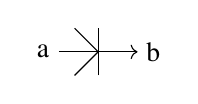
\begin{tikzpicture}
\draw[->] (0,0) -- (1,0);
\draw (0.5,-0.3) -- (0.5,0.3);
\draw (0.2,0.3) -- (0.5,0);
\draw (0.2,-0.3) -- (0.5,0);
\node at (-0.2,0) {a};
\node at (1.2,0) {b};
\end{tikzpicture}


\item  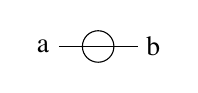
\begin{tikzpicture}
\draw (0,0) -- (1,0);
\draw (0.5,0) circle (0.2);
\node at (-0.2,0) {a};
\node at (1.2,0) {b};
\end{tikzpicture}


\item  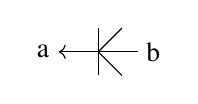
\begin{tikzpicture}
\draw[->] (1,0) -- (0,0);
\draw (0.5,-0.3) -- (0.5,0.3);
\draw (0.8,0.3) -- (0.5,0);
\draw (0.8,-0.3) -- (0.5,0);
\node at (-0.2,0) {a};
\node at (1.2,0) {b};
\end{tikzpicture}


\item 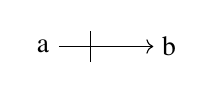
\begin{tikzpicture}
\draw (0,0) -- (0.4,0);
\draw (0.4,-0.2) -- (0.4,0.2);
\draw (0.4,0) -- (0.8,0);
\draw[->] (0.8,0) -- (1.2,0);
\node at (-0.2,0) {a};
\node at (1.4,0) {b};
\end{tikzpicture}
 \end{enumerate}


\item The two inputs of a CRO are fed with two stationary periodic signals. In the X-Y mode, the screen shows a figure which changes from ellipse to circle and back to ellipse with its major axis changing orientation slowly and repeatedly. The following inference can be made from this. 
\hfill(GATE EE 2009)
\begin{enumerate}
    \item  The signals are not sinusoidal 
\item  The amplitudes of the signals are very close but not equal 
\item  The signals are sinusoidal with their frequencies very close but not equal 
\item There is a constant but small phase difference between the signals
\end{enumerate}


\item The increasing order of speed of data access for the following devices is

(i) Cache Memory \quad (ii) CDROM \quad (iii) Dynamic RAM \quad (iv) Processor Registers \quad (v) Magnetic Tape 
\hfill(GATE EE 2009)
\begin{enumerate}
    \item  (v), (ii), (iii), (iv), (i) 
\item  (v), (ii), (iii), (i), (iv) 
\item  (ii), (i), (iii), (iv), (v) 
\item  (v), (ii), (i), (iii), (iv)
\end{enumerate}


\item A field excitation of $20 A$ in a certain alternator results in an armature current of $400 A$ in short circuit and a terminal voltage of 2000 V on open circuit. The magnitude of the internal voltage drop within the machine at a load current of 200 A is 
\hfill(GATE EE 2009)
\begin{enumerate}
\item  1 V 
\item  10 V 
\item 100 V 
\item 1000 V
\end{enumerate}

\item The current through the $2 k \ohm$ resistance in the circuit shown is
\hfill(GATE EE 2009)
\begin{figure}[H]
    \centering
    \includegraphics[width=0.5\columnwidth]{figs/image.png}
    \caption{}
    \label{fig:placeholder}
\end{figure}

\begin{enumerate}
    \item  0 mA  
\item  1 mA  
\item  2 mA  
\item  6 mA

\end{enumerate}

\item Out of the following plant categories 
(i) Nuclear  (ii) Run-of-river  (iii) Pump Storage  (iv) Diesel 
the base load power plants are 
\hfill(GATE EE 2009)
\begin{enumerate}
    \item  (i) and (ii) 
\item  (ii) and (iii) 
\item  (i), (ii) and (iii) 
\item  (i), (iii) and (iv)
\end{enumerate}

\item For a fixed value of complex power flow in a transmission line having a sending end voltage $V$, the real power loss will be proportional to 
\hfill(GATE EE 2009)
\begin{enumerate}
\item  $V$  
\item  $V^2$  
\item  $1/V^2$  
\item  $1/V$ 
\end{enumerate}


\item How many 200W/220V incandescent lamps connected in series would consume the same total power as a single 100W/220V incandescent lamp?
\hfill(GATE EE 2009)
\begin{enumerate}
    \item not possible
    \item 4
    \item 3
    \item 2
\end{enumerate}


\item A Linear Time Invariant system with an impulse response $h(t)$ produces output $y(t)$ when input $x(t)$ is applied. When the input $x(t-\tau)$ is applied to a system with impulse response $h(t-\tau)$, the output will be
\hfill(GATE EE 2009)
\begin{enumerate}
    \item  $y(t)$
    \item $y(2(1-t))$
    \item $y(t-\tau)$
    \item $y(t-2\tau)$
\end{enumerate}


\item The nature of feedback in the opamp circuit shown is
\hfill(GATE EE 2009)
\begin{figure}[h]

    \centering
    \includegraphics[width=0.5\columnwidth]{figs/Screenshot 2025-08-08 182804.png}
    \caption{}
    \label{fig:placeholder}
\end{figure}

\begin{enumerate}
    \item Current - Current feedback
    \item Voltage - Voltage feedback
    \item Current - Voltage feedback
    \item Voltage - Current feedback
\end{enumerate}



\item The complete set of only those Logic Gates designated as Universal Gates is
\hfill(GATE EE 2009)
\begin{enumerate}
     \item NOT, OR and AND Gates
     \item XNOR,NOR and NAND Gates
     \item NOR and NAND Gates
     \item XOR,  NOR and NAND Gates
\end{enumerate}


\item The single phase, 50Hz, iron core transformer in the circuit has both the vertical arms of cross sectional area $20\text{ cm}^2$ and both the horizontal arms of cross sectional area $10\text{ cm}^2$. If the two windings shown were wound instead on opposite horizontal arms, the mutual inductance will
\hfill(GATE EE 2009)
\begin{figure}[h]
    \centering
    \includegraphics[width=0.5\columnwidth]{figs/Screenshot 2025-08-08 191933.png}
    \caption{}
    \label{fig:placeholder}
\end{figure}

\begin{enumerate}
    \item double
     \item remain same
     \item be halved
     \item become one quarter
\end{enumerate}


\item A 3-phase squirrel cage induction motor supplied from a balanced 3-phase source drives a mechanical load. The torque-speed characteristics of the motor (solid curve) and of the load (dotted curve) are shown.Of the two equilibrium points A and B, which of the following options correctly describes the stability of A and B?
\hfill(GATE EE 2009)
\begin{figure}[h!]
    \centering
    \includegraphics[width=0.5\columnwidth]{figs/Screenshot 2025-08-08 191438.png}
    \caption{}
    \label{fig:placeholder}
\end{figure}

\begin{enumerate}
    \item A is stable, B is unstable
    \item A is unstable, B is stable
    \item Both are stable
    \item Both are unstable
\end{enumerate}


\item An SCR is considered to be a semi-controlled device because
\hfill(GATE EE 2009)
\begin{enumerate}
    \item it can be turned OFF but not ON with a gate pulse
    \item it conducts only during one half-cycle of an alternating current wave
    \item it can be turned ON but not OFF with a gate pulse
    \item it can be turned ON only during one half-cycle of an alternating voltage wave
\end{enumerate}


\item The polar plot of an open loop stable system is shown below. The closed loop system is
\hfill(GATE EE 2009)
\begin{figure}[h!]
    \centering
    \includegraphics[width=0.5\columnwidth]{figs/Screenshot 2025-08-08 192713.png}
    \caption{}
    \label{fig:placeholder}
\end{figure}

\begin{enumerate}
    \item always stable
    \item marginally stable
    \item unstable with one pole on the right half $s$-plane
    \item unstable with two poles on the right half $s$-plane
\end{enumerate}


\item The first two rows of Routh's tabulation of a third order equation are as follows:
\hfill(GATE EE 2009)
\[
\begin{array}{ccc}
s^3 & 2 & 2 \\
s^2 & 4 & 4
\end{array}
\]
This means there are
\begin{enumerate}
    \item  two roots at $s = \pm j$ and one root in right half $s$-plane
    \item two roots at $s = \pm j2$ and one root in left half $s$-plane
      \item two roots at $s = \pm j2$ and one root in right half $s$-plane
     \item  two roots at $s = \pm j$ and one root in left half $s$-plane
\end{enumerate}



\item The asymptotic approximation of the log-magnitude vs frequency plot of a system containing only real poles and zeros is shown. Its transfer function is
\hfill(GATE EE 2009)
\begin{figure}[h!]
    \centering
    \includegraphics[width=0.5\columnwidth]{figs/Screenshot 2025-08-08 194719.png}
    \caption{}
    \label{fig:placeholder}
\end{figure}

\begin{enumerate}
     \item  $\dfrac{10(s+5)}{s (s+2) (s+25)}$
     \item  $\dfrac{1000 (s+5)}{s^{2} (s+2)(s+25)}$
 \item  $\dfrac{100 (s+5)}{s (s+2) (s+25)}$
     \item $\dfrac{80 (s+5)}{s^{2} (s+2) (s+25)}$
\end{enumerate}



\item The trace and determinant of a $2 \times 2$ matrix are known to be $-2$ and $-35$ respectively. Its eigenvalues are
\hfill(GATE EE 2009)
\begin{enumerate}
     \item  $-30$ and $-5$
     \item  $-37$ and $-1$
     \item $-7$ and $5$
     \item $17.5$ and $-2$
\end{enumerate}

\item The following circuit has $R = 10\,\text{k} \ohm$, $C = 10\,\mu\text{F}$. The input voltage is a sinusoid at 50 Hz with an rms value of 10 V. Under ideal conditions, the current from the source is
\hfill(GATE EE 2009)
\begin{figure}[h!]
    \includegraphics[width=0.35\columnwidth]{figs/Screenshot 2025-08-08 200039.png}
    \caption{}
    \label{fig:placeholder}
\end{figure}

\begin{enumerate}
    \item $10 \pi\,\text{mA}$ leading by $90\degree$
    \item $20 \pi\,\text{mA}$ leading by $90\degree$
    \item $10\,\text{mA}$ leading by $90\degree$
    \item $10 \pi\,\text{mA}$ lagging by $90\degree$
\end{enumerate}


\item In the figure shown, all elements used are ideal. For time $t < 0$, $S_1$ remained closed and $S_2$ open. At $t=0$, $S_1$ is opened and $S_2$ is closed. If the voltage $V_{C2}$ across the capacitor $C_2$ at $t=0^{-}$ is 3 V, the voltage across the capacitor combination at $t=0^{+}$ will be
\hfill(GATE EE 2009)
\begin{figure}[h!]
    \centering
    \includegraphics[width=0.5\columnwidth]{figs/Screenshot 2025-08-08 200324.png}
    \caption{}
    \label{fig:placeholder}
\end{figure}
\begin{enumerate}
    \item 1 V
    \item 2 V
    \item 1.5 V
    \item 3 V
\end{enumerate}

\item Transformer and emitter follower can both be used for impedance matching at the output of an audio amplifier. The basic relationship between the input power $P_{\text{in}}$ and output power $P_{\text{out}}$ in both the cases is
\hfill(GATE EE 2009)
\begin{enumerate}
    \item $P_{\text{in}} = P_{\text{out}}$ for both transformer and emitter follower
    \item $P_{\text{in}} > P_{\text{out}}$ for both transformer and emitter follower
    \item $P_{\text{in}} < P_{\text{out}}$ for transformer and $P_{\text{in}} = P_{\text{out}}$ for emitter follower
    \item $P_{\text{in}} = P_{\text{out}}$ for transformer and $P_{\text{in}} < P_{\text{out}}$ for emitter follower
\end{enumerate}



\item The equivalent capacitance of the input loop of the circuit shown is
\hfill(GATE EE 2009)
\begin{figure}[h!]
    \centering
    \includegraphics[width=0.5\columnwidth]{figs/Screenshot 2025-08-08 202455.png}
    \caption{}
    \label{fig:placeholder}
\end{figure}



\begin{enumerate}
    \item $2\ \mu F$
    \item $100\ \mu F$
    \item $200\ \mu F$
    \item $4\ \mu F$
\end{enumerate}

\item In an 8085 microprocessor, the contents of the Accumulator, after the following instructions are executed, will become
\hfill(GATE EE 2009)

\begin{tabular}{l}
XRA A \\
MVIB F0H \\
SUB B
\end{tabular}

\begin{enumerate}
    \item $01\text{H}$
    \item $0F\text{H}$
    \item $F0\text{H}$
    \item $10\text{H}$
\end{enumerate}


\item For the Y-bus matrix of a 4-bus system given in per unit, the buses having shunt elements are

\hfill(GATE EE 2009)
$Y_{\text{BUS}} = \mathrm{j}\myvec{
-5 & 2 & 2.5 & 0 \\
2 & -10 & 2.5 & 4 \\
2.5 & 2.5 & -9 & 4 \\
0 & 4 & 4 & -8
}$


\begin{enumerate}
    \item 3 and 4
    \item 2 and 3
    \item 1 and 2
    \item 1, 2 and 4
\end{enumerate}

\item The unit-step response of a unity feedback system with open loop transfer function 

\begin{align*}
G(s)&= \frac{K}{(s+1)(s+2)}
\end{align*}

is shown in the figure. The value of $K$ is

\hfill(GATE EE 2009)
\begin{figure}[h!]
    \centering
    \includegraphics[width=0.5\columnwidth]{figs/Screenshot 2025-08-08 203002.png}
    \caption{}
    \label{fig:placeholder}
\end{figure}

\begin{enumerate}
    \item 0.5
    \item 2
    \item 4
    \item 6
\end{enumerate}


\item The open loop transfer function of a unity feedback system is given by

\begin{align*}
G(s)&= \frac{e^{-0.1s}}{s} 
\end{align*}

The gain margin of this system is
\hfill(GATE EE 2009)
\begin{enumerate}
    \item 11.95 dB
    \item 17.67 dB
    \item 21.33 dB
    \item 23.9 dB
\end{enumerate}

\item Match the items in List-I with the items in List-II and select the correct answer using the codes given below the lists.
\hfill(GATE EE 2009)
\begin{tabular}{ll}
\textbf{List I} & \textbf{List II}\\
a. improve power factor & 1. shunt reactor \\
b. reduce the current ripples & 2. shunt capacitor \\
c. increase the power flow in line & 3. series capacitor \\
d. reduce the Ferranti effect & 4. series reactor \\
\end{tabular}



\begin{enumerate}
    \item a - 2, b - 3, c - 4, d - 1
    \item a - 2, b - 4, c - 3, d - 1
    \item a - 4, b - 3, c - 1, d - 2
    \item a - 4, b - 1, c - 3, d - 2
\end{enumerate}


\item Match the items in List-I with the items in List-II and select the correct answer using the codes given below the lists.
\hfill(GATE EE 2009)
\begin{tabular}{ll}
\textbf{List I} & \textbf{List II}\\
a. Short Line & 1. Ohm Relay \\
b. Medium Line & 2. Reactance Relay \\
c. Long Line & 3. Mho Relay \\
\end{tabular}



\begin{enumerate}
    \item a - 2, b - 1, c - 3
    \item a - 3, b - 2, c - 1
    \item a - 1, b - 2, c - 3
    \item a - 1, b - 3, c - 2
\end{enumerate}


\item Three generators are feeding a load of 100 MW. The details of the generators are:
\hfill(GATE EE 2009)
\begin{tabular}{lccc}
\textbf{Rating (MW)} & \textbf{Efficiency (\%)} & \textbf{Regulation (p.u.) on 100 MVA base} \\
Generator-1 & 100 & 20 & 0.02 \\
Generator-2 & 100 & 30 & 0.04 \\
Generator-3 & 100 & 40 & 0.03 \\
\end{tabular}



In the event of increased load power demand, which of the following will happen?
\hfill(GATE EE 2009)
\begin{enumerate}
    \item All the generators will share equal power
    \item Generator-3 will share more power compared to Generator-1
    \item Generator-1 will share more power compared to Generator-2
    \item Generator-2 will share more power compared to Generator-3
\end{enumerate}



\item A 500 MW, 21 kV, 50 Hz, 3-phase, 2-pole synchronous generator having a rated power factor $= 0.9$, has a moment of inertia of $27.5 \times 10^{3}$ kg-m$^{2}$. The inertia constant ($H$) will be
\hfill(GATE EE 2009)
\begin{enumerate}
    \item 2.44 s
    \item 2.71 s
    \item 4.88 s
    \item 5.42 s
\end{enumerate}


\item $f(x, y)$ is a continuous function defined over $(x,y) \in [0,1]\times[0,1]$. Given the two constraints, $x > y^{2}$ and $y > x^{2}$, the volume under $f(x,y)$ is
\hfill(GATE EE 2009)
\begin{enumerate}
    \item $\displaystyle \int_{0}^{1} \int_{y^{2}}^{1} f(x,y) \, dx \, dy$
    \item $\displaystyle \int_{0}^{1} \int_{x^{2}}^{1} f(x,y) \, dy \, dx$
    \item $\displaystyle \int_{0}^{1} \int_{0}^{\sqrt{x}} f(x,y) \, dy \, dx$
    \item $\displaystyle \int_{0}^{1} \int_{0}^{\sqrt{y}} f(x,y) \, dx \, dy$
\end{enumerate}


\item Assume for simplicity that $N$ people, all born in April (a month of 30 days), are collected in a room. Consider the event of at least two people in the room being born on the same date of the month, even if in different years, e.g. 1980 and 1985. What is the smallest $N$ so that the probability of this event exceeds 0.5?
\hfill(GATE EE 2009)
\begin{enumerate}
    \item 20
    \item 7
    \item 15
    \item 16
\end{enumerate}



\item A cascade of 3 Linear Time Invariant systems is causal and unstable. From this, we conclude that
\hfill(GATE EE 2009)
\begin{enumerate}
    \item Each system in the cascade is individually causal and unstable
    \item At least one system is unstable and at least one system is causal
    \item At least one system is causal and all systems are unstable
    \item The majority are unstable and the majority are causal
\end{enumerate}


\item The Fourier Series coefficients, of a periodic signal $x(t)$, expressed as
\begin{align*}
x(t) = \sum_{k = -\infty}^\infty a_k e^{j 2 \pi k t / T}
\end{align*}
are given by:
\hfill(GATE EE 2009)
\begin{align*}
a_{-2} = 2 - j1, \quad a_{-1} = 0.5 + j0.2, \quad a_{0} = j2, \quad a_{1} = 0.5 - j0.2, \quad a_{2} = 2 + j1, \quad a_k = 0 \quad \text{for } |k| > 2.
\end{align*}

Which of the following is true?
\hfill(GATE EE 2009)
\begin{enumerate}
    \item $x(t)$ has finite energy because only finitely many coefficients are non-zero
    \item $x(t)$ has zero average value because it is periodic
    \item The imaginary part of $x(t)$ is constant
    \item The real part of $x(t)$ is even
\end{enumerate}


\item The z-transform of a signal $x[n]$ is given by
\begin{align*}
4 z^{3} + 3 z^{-1} + 2 - 6 z^{2} + 2 z^{3}.
\end{align*}
It is applied to a system with a transfer function 
\begin{align*}
H(z) = 3 z^{-1} - 2.
\end{align*}
Let the output be $y(n)$. Which of the following is true?
\hfill(GATE EE 2009)
\begin{enumerate}
    \item $y(n)$ is non causal with finite support
    \item $y(n)$ is causal with infinite support
    \item $y(n) = 0$ for $|n| > 3$
    \item \(\mathrm{Re}[Y(z)]_{z = e^{j \theta}} = - \mathrm{Re}[Y(z)]_{z = e^{-j \theta}}, \quad \mathrm{Im}[Y(z)]_{z = e^{j \theta}} = \mathrm{Im}[Y(z)]_{z = e^{-j \theta}}, \quad -\pi \leq \theta < \pi\)
\end{enumerate}


\item A cubic polynomial with real coefficients
\hfill(GATE EE 2009)
\begin{enumerate}
    \item can possibly have no extrema and no zero crossings
    \item may have up to three extrema and up to two zero crossings
    \item cannot have more than two extrema and more than three zero crossings
    \item will always have an equal number of extrema and zero crossings
\end{enumerate}


\item Let 
\begin{align*}
(x^{2} - 117 = 0)
\end{align*}. 
The iterative steps for the solution using Newton-Raphson's method is given by
\hfill(GATE EE 2009)
\begin{enumerate}
      \item
   \begin{align*}
     (x_{k+1} = \frac{1}{2} \left(x_k + \frac{117}{x_k}\right))
    \end{align*}
    \item 
  \begin{align*}
       (x_{k+1} = x_k - \frac{117}{x_k})
       \end{align*}
       \item
  \begin{align*}
    (x_{k+1} = x_k - \frac{x_k}{117})
    \end{align*}
   \item
   \begin{align*}
        (x_{k+1} = x_k - \frac{1}{2} \left(x_k + \frac{117}{x_k}\right))
        \end{align*}
\end{enumerate}

\item \begin{align*}
\mathbf{F}(x,y) = (x^{2} + xy) \hat{a}_x + (y^{2} + xy) \hat{a}_y.
\end{align*}
Its line integral over the straight line from \((x,y) = (0,2)\) to \((2,0)\) evaluates to:
\hfill(GATE EE 2009)
\begin{enumerate}
    \item $-8$
    \item $4$
    \item $8$
    \item $0$
\end{enumerate}



\item An ideal opamp circuit and its input waveform are shown in the figures. The output waveform of this circuit will be:
\hfill(GATE EE 2009)

\begin{center}
    \includegraphics[width=0.7\columnwidth]{figs/Screenshot 2025-08-08 214119.png}
  \label{fig:placeholder}

\end{center}

\begin{enumerate}
    \item (Waveform A) \\
    \includegraphics[width=0.4\columnwidth]{figs/Screenshot 2025-08-08 214145.png}
    \item (Waveform B) \\
    \includegraphics[width=0.4\columnwidth]{figs/Screenshot 2025-08-08 214154.png}
    \item (Waveform C) \\
    \includegraphics[width=0.4\columnwidth]{figs/Screenshot 2025-08-08 214200.png}
    \item (Waveform D) \\
    \includegraphics[width=0.4\columnwidth]{figs/Screenshot 2025-08-08 214204.png}
\end{enumerate}

\item A 220 V, 50 Hz, single-phase induction motor has the following connection diagram and winding orientations shown. MM' is the axis of the main stator winding (M\textsubscript{1}M\textsubscript{2}), and AA' is that of the auxiliary winding (A\textsubscript{1}A\textsubscript{2}). Directions of the winding axes indicate direction of flux when currents in the windings are in the directions shown. Parameters of each winding are indicated. When switch $S$ is closed, the motor:
\hfill(GATE EE 2009)
\begin{center}
\centering
    \includegraphics[width=0.5\columnwidth]{figs/Screenshot 2025-08-08 214242.png}
    \label{fig:placeholder}

\end{center}

\begin{enumerate}
    \item rotates clockwise
    \item rotates anticlockwise
    \item does not rotate
    \item rotates momentarily and comes to a halt
\end{enumerate}




\item The circuit shows an ideal diode connected to a pure inductor and driven by a purely sinusoidal 50 Hz voltage source. The voltage source is 

\begin{align*}
v_s = 10 \sin(100 \pi t).
\end{align*}
\begin{figure}[h!]
    \centering
    \includegraphics[width=0.5\columnwidth]{figs/Screenshot 2025-08-08 215519.png}
\label{fig:placeholder}
\caption{}
\end{figure}

Under ideal conditions, the current waveform through the inductor will look like:
\hfill(GATE EE 2009)
\begin{enumerate}
        \item \includegraphics[width=0.4\columnwidth]{figs/Screenshot 2025-08-08 215542.png}
    \item \includegraphics[width=0.4\columnwidth]{figs/Screenshot 2025-08-08 215551.png} 
    \item \includegraphics[width=0.4\columnwidth]{figs/Screenshot 2025-08-08 215529.png} 
   \item  \includegraphics[width=0.4\columnwidth]{figs/Screenshot 2025-08-08 215536.png} 
\end{enumerate}

\item The current source inverter shown in the figure is operated by alternately turning on thyristor pairs (T1, T2) and (T3, T4). If the load is purely resistive, the theoretical maximum output frequency obtainable will be:

\hfill(GATE EE 2009)
\begin{figure}[H]
    \centering
  \includegraphics[width=0.7\columnwidth]{figs/Screenshot 2025-08-08 215620.png}
     \caption{}
    \label{fig:placeholder}
\end{figure}
  

\begin{enumerate}
    \item 125 kHz
    \item 250 kHz
    \item 500 kHz
    \item 50 kHz
\end{enumerate}


\item In the chopper circuit shown, the main thyristor (TM) is operated at a duty ratio of 0.8 which is much larger than the commutation interval.
If the maximum allowable reapplied dv/dt on \(T_M\) is \(50~\mathrm{V/\mu s}\), what should be the theoretical minimum value of \(C_1\)?
Assume current ripple through \(L_0\) to be negligible.
\hfill(GATE EE 2009)
\begin{figure}[h!]
    \centering
    \includegraphics[width=0.5\columnwidth]{figs/Screenshot 2025-08-09 101310.png}
    \label{fig:13}
\end{figure}

\begin{enumerate}
    \item  $0.2~\mu\mathrm{F}$
\item  $0.02~\mu\mathrm{F}$  
\item  $2~\mu\mathrm{F}$ 
\item  $20~\mu\mathrm{F}$ 
\end{enumerate}


\item Match the switch arrangements on the top row to the steady-state V-I characteristics on the lower row.
The steady-state operating points are shown by large black dots.
\hfill(GATE EE 2009)


\begin{figure}[h]
    \centering
    \includegraphics[width=0.5\columnwidth]{figs/Screenshot 2025-08-09 102009.png}
    \label{fig:placeholder}
\end{figure}




\begin{enumerate}
     \item  A-I, B-II, C-III, D-IV
    \item  A-II, B-IV, C-I, D-III
    \item  A-IV, B-III, C-I, D-II
    \item  A-IV, B-III, C-II, D-I
\end{enumerate}



\item For the circuit shown, find out the current flowing through the $2 \ohm$ resistance.
Also, identify the changes to be made to double the current flow through the $2\ohm$ resistance.
\hfill(GATE EE 2009)
\begin{figure}[h!]
    \centering
    \includegraphics[width=0.5\columnwidth]{figs/Screenshot 2025-08-09 102019.png}
    \caption{*}
    \label{fig:placeholder}
\end{figure}

\begin{enumerate}
    

\item (5A; Put $V_s = 20$V) 
\item  (2A; Put $V_s = 8$V) 
\item  (5A; Put $I_s = 10$A) 
\item  (7A; Put $I_s = 12$A) 
\end{enumerate}
 

\item The figure shows a three-phase delta connected load supplied from a \(\,400 \, \mathrm{V}\),
\(50\, \mathrm{Hz}\), 3-phase balanced source. The pressure coil (PC) and current coil (CC) of a wattmeter are
connected to the load as shown, with the coil polarities suitably selected to ensure a positive deflection.


\begin{figure}[H]
    \centering
    \includegraphics[width=0.5\columnwidth]{figs/Screenshot 2025-08-09 102914.png}
    \caption{*}
    \label{fig:placeholder}
\end{figure}
The wattmeter reading will be:
\hfill(GATE EE 2009)
\begin{enumerate}
    
\item 0 
\item 1600 W 
\item 800 W 
\item 400 W
\end{enumerate}


\item An average-reading digital multimeter reads \(10 \, \mathrm{V}\) when fed with a triangular wave,
symmetric about the time-axis. For the same input, an rms-reading meter will read:
\hfill(GATE EE 2009)
\begin{enumerate}
    

\item \(\dfrac{20}{\sqrt{3}}\) 
\item \(\dfrac{10}{\sqrt{3}}\) 
\item \(20\sqrt{3}\) 
\item  \(10\sqrt{3}\)
\end{enumerate}

\item  The figure shows the extended view of a 2-pole DC machine with 10 armature conductors.
Normal brush positions are shown by \(A\) and \(B\), placed at the interpolar axis. If the brushes are now 
shifted, in the direction of rotation, to \(A'\) and \(B'\) as shown, the voltage waveform \(V_{A'B'}\) will resemble:
\hfill(GATE EE 2009)
\begin{figure}[h!]
    \centering
    \includegraphics[width=0.5\columnwidth]{figs/Screenshot 2025-08-09 104422.png}
    \label{fig:placeholder}
    \caption{rotation speed at $\omega$ rad/sec}
\end{figure}

\begin{enumerate}
     

\item  \includegraphics[width=0.3\columnwidth]{figs/Screenshot 2025-08-09 104456.png} 
\item  \includegraphics[width=0.3\columnwidth]{figs/Screenshot 2025-08-09 104451.png} 
\item  \includegraphics[width=0.3\columnwidth]{figs/Screenshot 2025-08-09 104444.png} 
\item  \includegraphics[width=0.3\columnwidth]{figs/Screenshot 2025-08-09 104436.png}
\end{enumerate}

\subsection*{Common Data Questions}

\textbf{Common Data for Questions 51 and 52:}

The star-delta transformer shown below\ is excited on the star side with a balanced, 4-wire, 3-phase, 
sinusoidal voltage supply of rated magnitude. The transformer is under no load condition.

\begin{center}
\includegraphics[width=0.5\columnwidth]{figs/Screenshot 2025-08-09 105450.png}
\label{fig:placeholder}
\end{center}

\item  With both \(S_1\) and \(S_2\) open, the core flux waveform will be:
\hfill(GATE EE 2009)
\begin{enumerate}
    
\item  a sinusoid at fundamental frequency 
\item  flat-topped with third harmonic 
\item  peaky with third-harmonic 
\item  none of these
\end{enumerate}

\item With \(S_2\) closed and \(S_1\) open, the current waveform in the delta winding will be:
\hfill(GATE EE 2009)
\begin{enumerate}
    

\item  a sinusoid at fundamental frequency 
\item  flat-topped with third harmonic 
\item  only third-harmonic 
\item none of these
\end{enumerate}


\textbf{Common Data for Questions 53 and 54:}

The circuit diagram shows a two-winding, lossless transformer with no leakage flux, 
excited from a current source \(i(t)\) whose waveform is also shown.
The transformer has a magnetizing inductance of \(\frac{400}{\pi}\ \mathrm{mH}\).

\begin{center}
\includegraphics[width=0.75\columnwidth]{figs/Screenshot 2025-08-09 105611.png}
\label{fig:placeholder}
\end{center}

\item The peak voltage across A and B, with \(S\) open, is:
\hfill(GATE EE 2009)
\begin{enumerate}
 
\item \(\frac{400}{\pi} \text{ V}\) 
\item  \(800 \ \text{V}\) 
\item  \(\frac{4000}{\pi} \ \text{V}\) 
\item  \(\frac{800}{\pi} \ \text{V}\)
\end{enumerate}

\item If the waveform of \( i(t) \) is changed to
\begin{align*}
i(t) = 10 \sin(100 \pi t) \ \text{A},
\end{align*}
the peak voltage across A and B with \( S \) closed is:
\hfill(GATE EE 2009)
\begin{enumerate}
    

\item \(400 \ \mathrm{V}\) 
\item \(240 \ \mathrm{V}\) 
\item \(320 \ \mathrm{V}\) 
\item  \(160 \ \mathrm{V}\)
\end{enumerate}

\textbf{Common Data for Questions 55 and 56}

A system is described by the following state and output equations:
\begin{align*}
\frac{dx_1(t)}{dt} = -3x_1(t) + x_2(t) + 2u(t)
\frac{dx_2(t)}{dt} = -2x_2(t) + u(t)
y(t) = x_1(t)
\end{align*}
where \(u(t)\) is the input and \(y(t)\) is the output.
 
\item  The system transfer function is:
\hfill(GATE EE 2009)
\begin{enumerate}
    
\item  \(\dfrac{s+2}{s^{2} + 5s - 6}\) 
\item  \(\dfrac{s+3}{s^{2} + 5s + 6}\) 
\item  \(\dfrac{2s+5}{s^{2} + 5s + 6}\)
\item  \(\dfrac{2s - 5}{s^{2} + 5s - 6}\)
\end{enumerate}

\item  The state-transition matrix of the above system is:
\hfill(GATE EE 2009)
\begin{enumerate}
\item \[ \myvec{
e^{-3t} & 0 \\
e^{-2t} + e^{-3t} & e^{-2t} } 
\]
\item \[ \myvec{
e^{-3t} & e^{-2t} - e^{-3t} \\
0 & e^{-2t} }
\]
\item \[\myvec{
e^{-3t} & e^{-2t} + e^{-3t} \\
0 & e^{-2t} } 
\]
\item \[ \myvec{
e^{-3t} & e^{-2t} - e^{-3t} \\
0 & e^{-2t} }
\]
\end{enumerate}



\textbf{Linked Answer Questions}

\textbf{Statement for Questions 57 and 58:}

The figure below shows coils 1 and 2, with dot markings as indicated, having \( 4000 \) and \( 6000 \) turns respectively.  
Both the coils have a rated current of \( 25 \ \mathrm{A} \).  
Coil 1 is excited with single-phase, \( 400 \ \mathrm{V},\ 50 \ \mathrm{Hz} \) supply.

\begin{center}
\includegraphics[width=0.6\columnwidth]{figs/Screenshot 2025-08-09 110459.png}
\label{fig:placeholder}
\end{center}
 
\item The coils are to be connected to obtain a single-phase, \(400/1000 \ \mathrm{V}\), auto-transformer to drive a load of \(10 \ \mathrm{kVA}\).  
Which of the options should be exercised to realize the required auto-transformer?
\hfill(GATE EE 2009)
\begin{enumerate}
\item Connect A and D; Common B 
\item Connect B and D; Common C 
\item  Connect A and C; Common B 
\item  Connect A and C; Common D
\end{enumerate}


\item In the autotransformer obtained in Question 57, the current in each coil is:
\hfill(GATE EE 2009)
\begin{enumerate}
    
\item  Coil-1 is \(25 \ \mathrm{A}\) and Coil-2 is \(10 \ \mathrm{A}\) 
\item  Coil-1 is \(10 \ \mathrm{A}\) and Coil-2 is \(25 \ \mathrm{A}\) 
\item  Coil-1 is \(10 \ \mathrm{A}\) and Coil-2 is \(15 \ \mathrm{A}\) 
\item Coil-1 is \(15 \ \mathrm{A}\) and Coil-2 is \(10 \ \mathrm{A}\)
\end{enumerate}

 
\subsection*{Linked Answer Questions}

\textbf{Statement for Questions 59 and 60:}

The circuit diagram is shown below:

\begin{center}
\includegraphics[width=0.6\columnwidth]{figs/Screenshot 2025-08-09 110647.png}
\label{fig:placeholder}
\end{center}

\item For the circuit given above, the Thevenin's resistance across the terminals A and B is:
\hfill(GATE EE 2009)
\begin{enumerate}
    

\item \(0.5 \ \mathrm{k\ohm}\) 
\item  \(0.2 \ \mathrm{k\ohm}\) 
\item  \(1 \ \mathrm{k\ohm}\) 
\item  \(0.11 \ \mathrm{k\ohm}\)
\end{enumerate} 

For the circuit given above, the Thevenin's voltage across the terminals A and B is:
\hfill(GATE EE 2009)
\begin{enumerate}
    

\item  \(1.25 \ \mathrm{V}\) 
\item  \(0.25 \ \mathrm{V}\) 
\item  \(1 \ \mathrm{V}\) 
\item  \(0.5 \ \mathrm{V}\)
\end{enumerate}


\begin{center}
\textbf{--- END OF THE QUESTION PAPER ---}
\end{center}

\end{enumerate}
\end{flushleft}
\end{document}

        


